\section{Introduction}
\label{sec:intro}

We introduce the new task of noun phrase linking, which annotates all noun phrases in a document with its corresponding entry in a knowledge base (such as Wikipedia). 
This task can be viewed as a generalization of Named Entity Linking (\nel{}), which matches named entities with entries in an external knowledge base. 
The task is more difficult than \nel{} because of the difficulty in resolving non-explicit references. 
The task is also related to, but separate from, coreference resolution, as it also deals with references to entities not present in the document, but only deals with noun phrases that link to an external knowledge base. 
\\
\\
Named entity linking is used in many downstream tasks, including question answering (QA) systems~\cite{yamada2018studio}. 
For example, in Figure 1, a question from Quizbowl (\qb{}), a trivia competition, is annotated with entities, such as "one work by this author" linking to Novum Organum. 
Expanding from \nel{} to noun phrase linking gives QA systems more information and offloads some of the difficulty of question answering from QA systems to the noun phrase linkers. 
We focus on \qb{} because Quizbowl questions have sophisticated noun phrases, because the queestions describe but don't explicitly mention named entities. 
Quizbowl questions average $21.2$ entities per question, which is more than other datasets, such as \triviaqa{} which only has $2.2$~\cite{zhao2020delft}.  
Replacing noun phrases with their respective entities allows for question answering systems to gain information, which changes the answer from David Hume, to the correct answer of Francis Bacon. 
\begin{figure}[t]
	\label{fig:fig1}
	\begin{center}
		\tikz\node[draw=black!40!lightblue,inner sep=1pt,line width=0.3mm,rounded corners=0.1cm]{ 			\begin{tabular}{p{.9\linewidth}}
								\underline{\color{blue} One work by this author} (Novum Organum) uses printing, gunpowder, and the compass as symbols of personal ambition, national ambition, and the ambition of the human race to extend its grasp. 
				\underline{\color{blue} This thinker} (Francis Bacon) described three forms of false learning as “delicate”, “contentious”, and “fantastical” in categorizing the “distempers” that impede academic progress. 
				\underline{\color{blue} This thinker} (Francis Bacon) imagined a utopian university called \underline{Salomon’s House} (Salomon's house), and \underline{he} (Francis Bacon) likened received systems of philosophy to stage plays that misrepresent the world, and thus labeled them \underline{“idols of the theatre”}(Idola Theatari). 
				This author of \underline{The New Atlantis} (New Atlantis) established the \underline{doctrine of inductive, empirical methodology} (Baconian method). 
				For 10 points, name \underline{\color{blue} this 17th-century English philosopher} (Francis Bacon) who wrote \underline{Novum Organum} (Novum Organum) and spearheaded the \underline{Scientific Revolution} (Scientific Revolution)\\
				\textbf{Answer:} \underline{Francis Bacon}
							\end{tabular}
		};
	
   \vspace{1.1cm}
	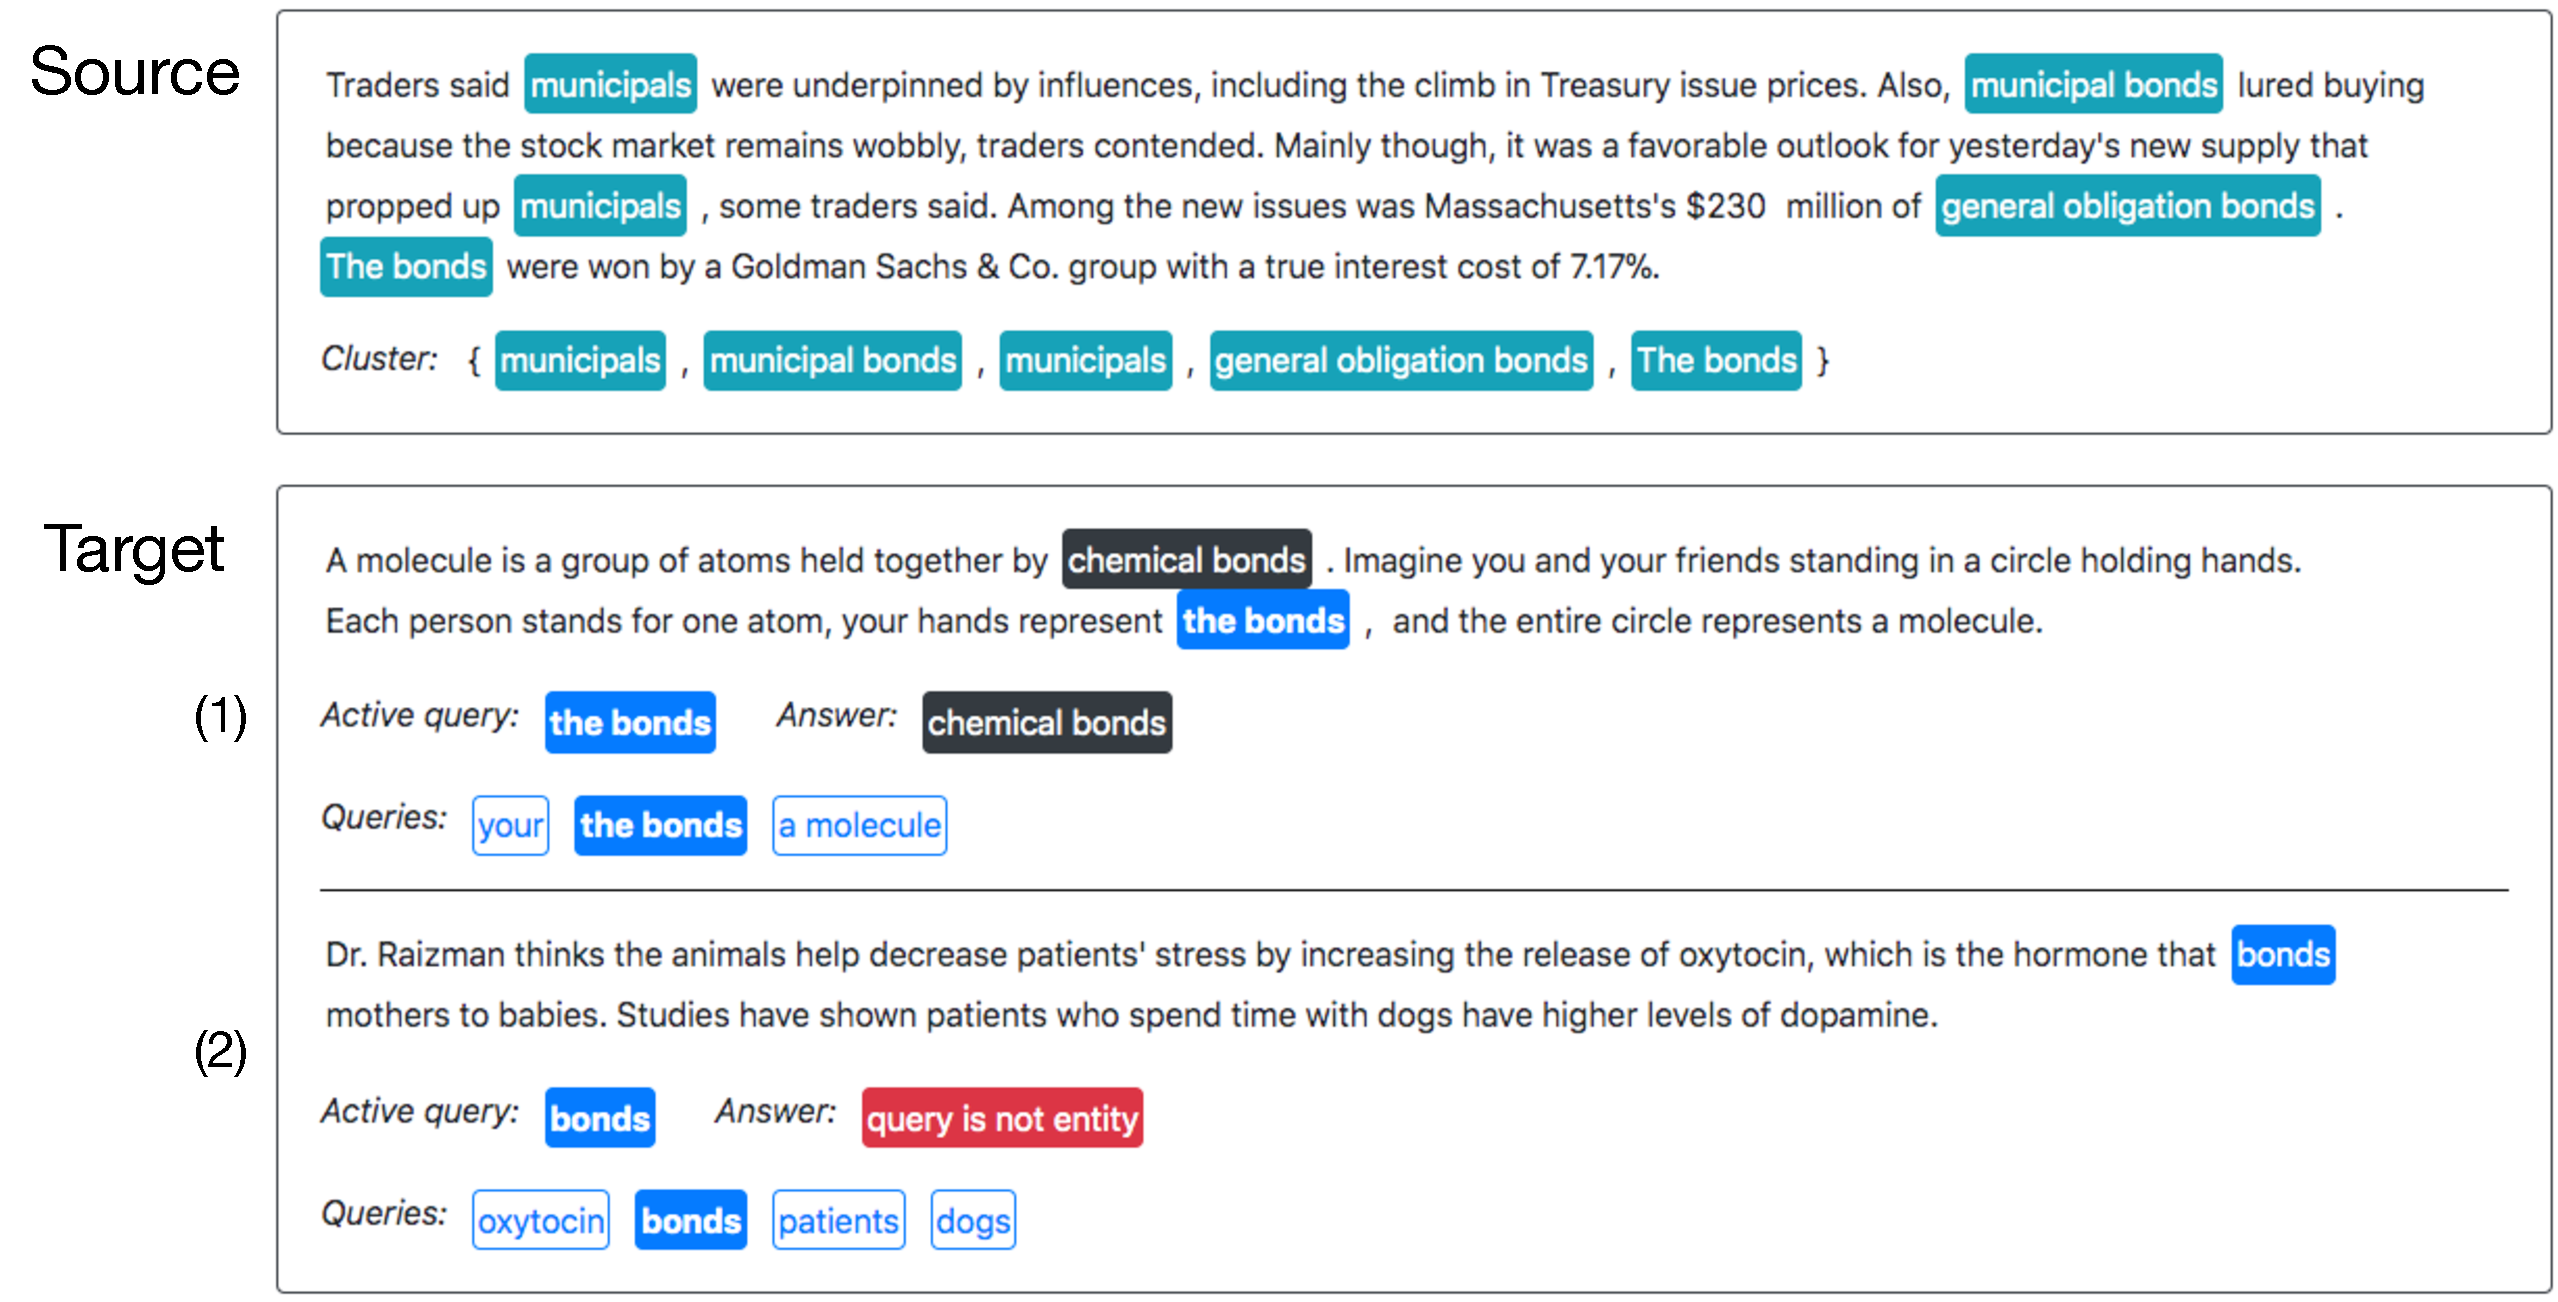
\includegraphics[width=\columnwidth]{example}
	\end{center}
	\caption{
		We show a \qb{} question with a variety of hard and easy entities; entities that would be linked only by a noun phrase linker are in blue. 
		Questions from this dataset are entity dense, and contain complex reference patterns, such as "doctrine of inductive, empirical methodology" linking to the Baconian method. 
		In general, we validate the utility of noun phrase linking for question answering by substituting noun phrases with their links and observe accuracy gains. 
		For example, replacing noun phrases in the first sentence changes the answer from the incorrect David Hume, to the correct Francis Bacon. 
	}

\end{figure}

Noun phrase linking is a more difficult task than named entity linking due to the difficulty of annotating non-explicit references, and thus presents a challenge when curating a dataset. 
This work describes a process to build a dataset of noun phrase annotations for challenging trivia questions like \qb{}~\citep{qb19} in Figure~ 1, Jeopardy!~\citep{dunn2017searchqa}, \triviaqa{}~\citep{joshi2017trivia}, and Quasar-T~\citep{dhingra2017quasar}.
Although building datasets is expensive and time-consuming, this is mitigated and quality is improved by incorporating prior entity linking models into the annotation process~\citep{wallace2018trick,dua2019drop,dasigi2019quoref,nie2019adversarial}.
Our key insight and the hypothesis we test is that the bias introduced by exposing human annotators to machine predictions is small in comparison to the increase in annotation coverage and quality.
To measure this, we plan to run an experiment where we vary the conditions in which the training data is annotated.
Specifically, we plan to vary which entity linking or coreference models are used to assist annotator, and analyze the difference in linking accuracy by the type of models used. 
\\
\\
We additionally plan to use human-in-the-loop annotation to suggest noun phrases to annotate along with the links for those phrases.
We motivate experts to annotate, in this case, trivia competitors and organizers, which improves annotation quality.
\\
\\
After collecting data, we design experiments to evaluate state of the art \nel{} and coreference models on noun phrase data. 
We collect a gold set and evaluate performance on that data set to determine the difficulty of annotating noun phrases when compared to general entity linking.
We develop a baseline noun phrase linking model based off of the dataset, which is trained through a human-in-the-loop process, and compare its performance against entity linkers and coreference models. 
We additionally develop experiments to determine the extent to which noun phrase linking assists with question answering. 
\\
\\
In summary, we make three contributions: (1) Define the new problem of noun phrase annotating, and show that annotating noun phrases improves \qa{} performance (2) Develop a method to collect noun phrase linking dataset using text from trivia datasets, (3) Propose experiments that evaluate current named entity linkers and coreference models on the noun phrase dataset, compare a baseline noun phrase model to entity linking and coreference, and evaluate the impact that noun phrase linking has upon question answering accuracy.
